%% ma: L12-B14-0006
%% lop: 12
%% chuong: 5
%% bai: 14
%% dang: 12.14.6
%% loai: TLN
%% muc: VD
%% dap_an: "5"
%% nguon: "(NBV)-ĐỀ SỐ 8-MỖI NGÀY 1 ĐỀ THI 2025.pdf (D08, MỖI NGÀY 1 ĐỀ - Đề số 8), Phần III Câu 2"
%% kien_thuc: "Bài 14 (phương trình mặt phẳng, vectơ pháp tuyến, tích có hướng), Bài 15/14 (giao tuyến, khoảng cách từ điểm đến mặt phẳng Oxy)"
%% trang_thai: cho-duyet
%% ly_do: "Dạng 12.14.6 (giao tuyến hai mặt phẳng: chiều cao nóc nhà) là dạng mới đề xuất."
%% ghi_chu: "Đáp án gốc 5 đúng (sympy: giao tuyến nằm ở độ cao z = 5). Lưu ý mô hình: mặt (P): x - 2y + 5 = 0 có vectơ pháp tuyến (1;-2;0) nằm ngang nên (P) là mặt phẳng thẳng đứng (không nghiêng như mái nhà trong hình gốc); hình TikZ vẽ minh họa mái hai phía, không theo tỉ lệ; đáp số vẫn là 5 theo phương trình."
\begin{ex}
Trong không gian $Oxyz$ (đơn vị trên mỗi trục tọa độ là mét), một ngôi nhà như hình vẽ dưới đây có sàn nhà nằm trên mặt phẳng $(Oxy)$. Hai mái nhà lần lượt nằm trên các mặt phẳng $(P):x-2y+5=0$ và $(Q):x-2y-3z+20=0$. Hỏi chiều cao của ngôi nhà tính từ sàn nhà lên nóc nhà (điểm cao nhất của mái nhà) là bao nhiêu?
\begin{center}
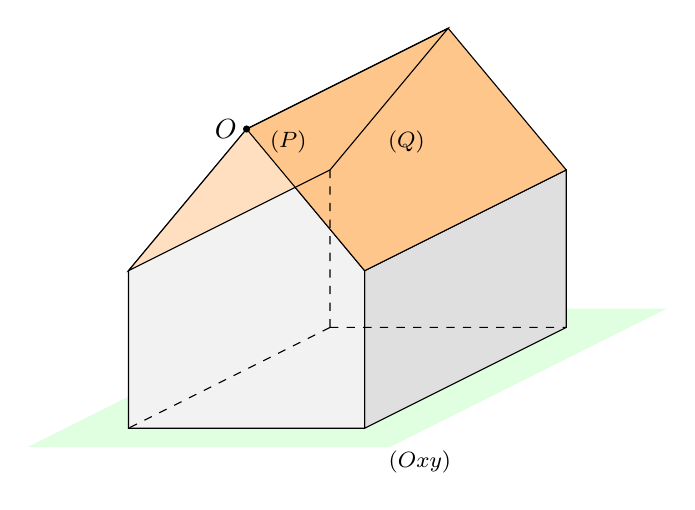
\begin{tikzpicture}[x={(-.8cm,-.4cm)},y={(1cm,0cm)},z={(0cm,1cm)}]
  \def\D{3.2}\def\W{3}\def\H{2}\def\R{3.8}
  \fill[green!12] (-.6,-.8,0)--(\D+.6,-.8,0)--(\D+.6,\W+.8,0)--(-.6,\W+.8,0)--cycle;
  \fill[gray!25] (0,\W,0)--(\D,\W,0)--(\D,\W,\H)--(0,\W,\H)--cycle;
  \draw (0,\W,0)--(\D,\W,0)--(\D,\W,\H)--(0,\W,\H)--cycle;
  \fill[gray!10] (\D,0,0)--(\D,\W,0)--(\D,\W,\H)--(\D,\W/2,\R)--(\D,0,\H)--cycle;
  \draw (\D,0,0)--(\D,\W,0)--(\D,\W,\H)--(\D,\W/2,\R)--(\D,0,\H)--cycle;
  \fill[orange!25] (0,0,\H)--(\D,0,\H)--(\D,\W/2,\R)--(0,\W/2,\R)--cycle;
  \fill[orange!45] (0,\W/2,\R)--(\D,\W/2,\R)--(\D,\W,\H)--(0,\W,\H)--cycle;
  \draw (0,0,\H)--(\D,0,\H)--(\D,\W/2,\R)--(0,\W/2,\R)--cycle;
  \draw (0,\W/2,\R)--(\D,\W/2,\R)--(\D,\W,\H)--(0,\W,\H)--cycle;
  \draw[dashed] (0,0,0)--(0,\W,0) (0,0,0)--(\D,0,0) (0,0,0)--(0,0,\H);
  \fill (\D,\W/2,\R) circle (1.3pt) node[left]{$O$};
  \node[font=\footnotesize] at (\D/2,\W/4,{(\H+\R)/2+.1}) {$(P)$};
  \node[font=\footnotesize] at (\D/2,{3*\W/4},{(\H+\R)/2+.1}) {$(Q)$};
  \node[font=\footnotesize,below right] at (\D+.4,\W+.5,0) {$(Oxy)$};
\end{tikzpicture}
\end{center}
\shortans{5}
\loigiai{Gọi $d$ là giao tuyến của $(P)$ và $(Q)$ (đường thẳng chứa nóc nhà). Vectơ pháp tuyến $\overrightarrow{n_P}=(1;-2;0)$, $\overrightarrow{n_Q}=(1;-2;-3)$ và $\left[\overrightarrow{n_P},\overrightarrow{n_Q}\right]=(6;3;0)$ nên $d$ có vectơ chỉ phương $\overrightarrow u=(2;1;0)$, do đó $d\parallel(Oxy)$.
Chiều cao của ngôi nhà bằng khoảng cách từ $d$ đến $(Oxy)$. Lấy $A(1;3;5)$ thuộc $d$ (thỏa cả hai phương trình: $1-6+5=0$ và $1-6-15+20=0$), ta có $d\left(A,(Oxy)\right)=\dfrac{|5|}{\sqrt1}=5$.
Vậy chiều cao ngôi nhà là $5$ m.}
\end{ex}
